\section{GIT vs. SVN}
%
\subsection{R�ckblick zu SVN}
\begin{frame}
  \frametitle{R�ckblick zu SVN}
  \tableofcontents[currentsection,currentsubsection]
\end{frame}
\begin{frame}
  \frametitle{R�ckblick zu SVN}
  \begin{itemize}
    \item Repository auf zentralem Server einrichten
    \item<2->Arbeitskopie auschecken
      \begin{itemize}
        \item<3->Warten
      \end{itemize}
    \item<4->Dateien zur Versionierung hinzuf�gen
      \begin{itemize}
        \item<5->Warten
      \end{itemize}
    \item<6->Commit
      \begin{itemize}
        \item<7->Warten
      \end{itemize}
  \end{itemize}
\end{frame}
\begin{frame}
  \frametitle{Workflow SVN}
  \begin{center}
    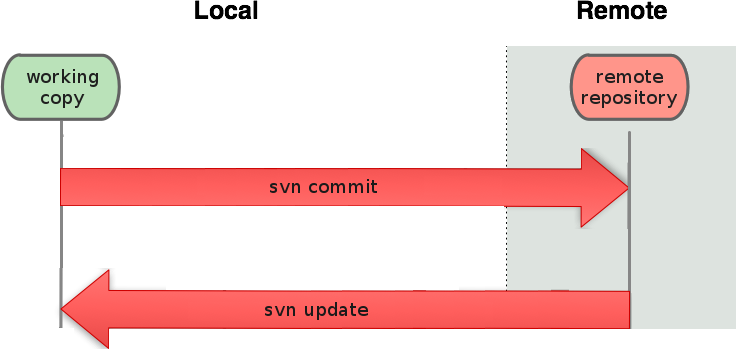
\includegraphics[width=0.95\textwidth]{images/local-remote-workflow-svn.png}
  \end{center}
\end{frame}
%
\subsection{Workflow mit GIT}
\begin{frame}
  \frametitle{Workflow mit GIT}
  \tableofcontents[currentsection,currentsubsection]
\end{frame}
\begin{frame}[fragile]
  \frametitle{Workflow mit GIT}
  \begin{itemize}
    \item Repository erstellen $\Leftrightarrow$ Arbeitskopie "`auschecken"'
      \begin{minted}[gobble=8]{sh}
        $ git init
      \end{minted}
    \item<2->Optional: Erzeugen einer \texttt{.gitignore}-Datei
    \item<3->Optional: Hinzuf�gen von Remotes
      \begin{minted}[gobble=8]{sh}
        $ git remote add origin git@thisdone.de:my_project.git
      \end{minted}
    \item<4->Dateien und �nderungen hinzuf�gen:
      \begin{minted}[gobble=8]{sh}
        $ git add .
      \end{minted}
    \item<5->Commit:
      \begin{minted}[gobble=8]{sh}
        $ git commit -m "Commit message"
      \end{minted}
    \item<6->Optional: Push auf Remote
      \begin{minted}[gobble=8]{sh}
        $ git push origin master
      \end{minted}
  \end{itemize}
\end{frame}
\begin{frame}
  \frametitle{Workflow mit GIT}
  \begin{center}
    \vspace{-7mm}
    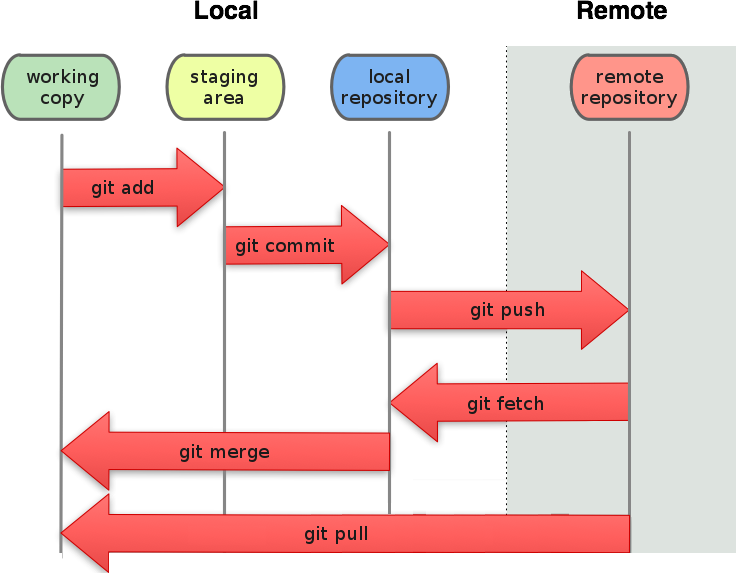
\includegraphics[height=.75\textheight]{images/local-remote-workflow-git.png}
  \end{center}
\end{frame}
%
\subsection{Tabellarischer Vergleich}
\begin{frame}
  \frametitle{Tabellarischer Vergleich}
  \tableofcontents[currentsection,currentsubsection]
\end{frame}
